\chapter{Background Research}\label{ch:background}

This chapter provides background context for the development of a liquid democracy system within vodle. It builds on the concepts introduced earlier, focusing on more detailed research into known limitations of liquid democracy and potential solutions proposed in academic literature. Additionally, the technical foundations and design philosophy of vodle as a platform are explored.

\section{Liquid Democracy}
As democratic participation increasingly shifts to online platforms, traditional models of governance face new constraints. Liquid democracy has emerged as a compelling alternative, combining the flexibility of direct voting with the scalability of delegation. It allows users to vote directly, delegate their vote to a trusted individual, or abstain entirely -- offering a dynamic and responsive approach to collective decision-making \citep{blum_liquid_2016}.

In a direct democracy, every individual casts their own vote on each issue. While this model provides maximum agency and transparency, it becomes impractical at scale due to the high cognitive and time demands placed on participants \citep{ford_delegative_2002}. Large or heterogeneous populations often feature varying levels of expertise, interest, and availability -- making sustained engagement unrealistic.

Representative democracy addresses scalability by electing officials to make decisions on behalf of others. However, this model can introduce misalignment between representatives and constituents, and voters lack the ability to adjust their preferences between elections \citep{blum_liquid_2016}.

Liquid democracy aims to resolve these tensions by enabling delegable, revocable proxy voting. Individuals can delegate their vote to someone they trust for a particular issue or domain, and change their delegation at any time. This empowers voters to participate as much or as little as they choose, without forfeiting influence.

The remainder of this chapter explores the practical challenges faced by liquid democracy (such as cycles, abstentions, and disproportionate influence) and introduce key enhancements like ranked delegation and vote splitting, which aim to address these limitations while preserving its flexibility and user control.

\subsection{Issues with Liquid Democracy -- TODO:INTRO}

While liquid democracy offers a flexible and adaptive alternative to traditional decision-making models, it also introduces distinct technical and social challenges. These arise from its reliance on transitive delegations and dynamic participation. In practice, unresolved issues such as delegation cycles, vote loss due to abstentions, and the emergence of disproportionately influential users (``super-voters'') can undermine both the fairness and effectiveness of the system. This section outlines these key issues, highlighting their impact on vote integrity and user trust.

\begin{table}[H]
  \centering
  \begin{tabular}{|@{}|l|l@{}|}
  \hline
  \textbf{Symbol} & \textbf{Role Description} \\ \hline
  \textbf{Circle}   & \textit{Delegated voter} -- has delegated their vote and does not cast one directly. \\
  \textbf{Square}   & \textit{Casting voter} -- casts their own vote and has not delegated. \\
  \textbf{Triangle} & \textit{Abstaining voter} -- neither delegates nor casts their own vote. \\
  \hline
  \end{tabular}
  \caption{Diagram symbol legend used to represent different voter behaviours.}
\end{table}  

\subsection*{Delegation Cycles}\label{subsec:delegation_cycles}
\begin{figure}[H]
  \centering
  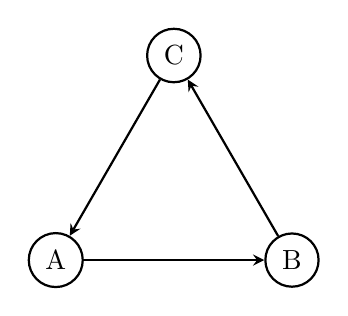
\begin{tikzpicture}[->, >=stealth, thick, scale=1.5]
    % Nodes at triangle vertices
    \node[circle, draw] (A) at (0,0) {A};
    \node[circle, draw] (B) at (2,0) {B};
    \node[circle, draw] (C) at (1,1.732) {C}; % height = sqrt(3)

    % Arrows showing delegation
    \draw (A) -- (B);
    \draw (B) -- (C);
    \draw (C) -- (A);
  \end{tikzpicture}
  \caption{Delegation cycle: A delegates to B, B to C, and C back to A.}
  \label{fig:triangle-cycle}
\end{figure}


Delegation cycles occur when a vote is delegated in such a way that it ends up forming a loop \citep{brill_liquid_2022}, preventing the vote from reaching a final casting voter. For example, if Alice delegates her vote to Bob, Bob delegates to Charlie, and Charlie delegates back to Alice, the votes become trapped in a cycle (seen above) and can be treated as a loss of representation \citep{christoff2017liquiddemocracyanalysisbinary}.

This issue is particularly problematic because it can nullify votes without the affected users ever realising. In systems where cycles are not explicitly detected and handled, these votes could be discarded silently, potentially changing the final outcome of the votes.

A simplistic method to prevent cycles is to check whether a delegation would create a cycle before allowing it. For example, if Alice tries to delegate her vote to Bob, the system checks whether Bob has already directly or indirectly delegated their vote to Alice. If so, the delegation is rejected. However, this approach can be cumbersome and may lead to a poor user experience, as users may not understand why their delegation was denied.

Delegation cycles are increasingly likely to emerge in dynamic voting systems, where delegations can be added, removed, or modified at any point in time. Delegations that initially did not form part of a cycle may later contribute to one as other voters add a new delegation or alter an existing one.
\subsection*{Abstentions}
\begin{figure}[H]
  \centering
  \begin{tikzpicture}[->, >=stealth, thick, node distance=2.5cm]
    \node[circle, draw] (A) {A};
    \node[circle, draw, right of=A] (B) {B};
    \node[regular polygon, regular polygon sides=3, shape border rotate=0, draw, minimum size=1cm, inner sep=0pt, right of=B] (C) {C};

    \draw (A) -- (B);
    \draw (B) -- (C);
  \end{tikzpicture}
  \caption{Delegation chain ending in abstention: A delegates to B, B to C. C abstains, causing the votes of A and B to be lost.}
  \label{fig:delegation-abstention}
\end{figure}

A voter abstains by neither casting a vote nor delegating it to another user \citep{brill_liquid_2022}. This includes both deliberate abstention, where a voter knowingly chooses not to participate, and passive abstention, where a voter may be unaware of an ongoing poll or are unable to engage with it.

Abstentions are especially impactful when they occur at the end of a larger delegation chain, as all votes passed along the chain to that voter are effectively lost \citep{brill_liquid_2022}. Additionally, the voters whose decisions were passed along the chain may also be unaware that their votes have been nullified, worsening the effect of the abstention.

\subsection*{Super-Voters}
\begin{figure}[h]
  \centering
  \begin{tikzpicture}[->, >=stealth, thick, node distance=2.5cm, square/.style={regular polygon,regular polygon sides=4}]
    \node[circle, draw] (A) {A};
    \node[circle, draw, right of=A] (B) {B};
    \node[square, draw, minimum size=1cm, inner sep=0pt, right of=B] (C) {C};
    \node[square, draw, minimum size=1cm, inner sep=0pt, right of=C] (D) {D};
    \node[square, draw, minimum size=1cm, inner sep=0pt, right of=D] (E) {E};

    \draw (A) -- (B);
    \draw (B) -- (C);
  \end{tikzpicture}
  \caption{Super-voter: A delegates to B, B to C. No matter which vote D or E cast, C's vote will always determine the outcome as it has a weight of 3.}
  \label{fig:delegation-supervoter}
\end{figure}

In liquid democracy, a \textit{super-voter} is a user who receives a large number of delegations, thereby accumulating significant voting power \citep{kling2015votingbehaviourpoweronline}. While such concentration may arise from genuine trust, it risks creating imbalances that contradict the egalitarian goals of the system. Super-voters can effectively act as unelected representatives -- potentially swaying results with little accountability.

Even when systems allow voters to revoke delegations at any time, many users may not actively monitor how their vote is used. This can lead to persistent power structures where a small number of users hold substantial, often unnoticed, influence over outcomes.

This phenomenon is not just theoretical. In the German Pirate Party's use of LiquidFeedback, some participants became so dominant that their votes carried decree-like weight, even though they were not formally elected \citep{sven_becker_liquid_2012, kling2015votingbehaviourpoweronline}. While \citet{kling2015votingbehaviourpoweronline} observed that these super-voters generally aligned with majority opinion -- contributing to system stability rather than distorting it -- their influence still raises concerns about transparency and voter autonomy.

Super-voting is not confined to traditional political platforms. In decentralised autonomous organisations (DAOs), which use token-based voting on blockchains, similar patterns emerge. \citet{hallWhatHappensWhen2024} found that in many DAOs, voting power was highly concentrated among a few delegates due to low participation. In some cases, such as Gitcoin, over 90\% of votes cast were controlled by the top five delegates.

These examples underscore the importance of delegation mechanisms that can curb excessive power accumulation. Techniques such as vote splitting and delegation caps are essential to preserving fairness, especially in systems like vodle that prioritise inclusivity and trust-based participation.

\subsection{Variations of Liquid Democracy}
The challenges discussed in the previous section, such as delegation cycles, vote loss due to abstentions, and the emergence of super-voters, highlight inherent vulnerabilities in the standard liquid democracy model. To mitigate these issues, enhancements have been proposed that modify how delegations function. These include techniques that allow voters to specify multiple delegates or distribute their vote to multiple casting voters. Each approach introduces different trade-offs and requires algorithmic support to ensure sound and interpretable outcomes.

The following subsections present several such variations, along with the algorithms that can be used to implement them.
\subsection*{Ranked Delegation}
Ranked delegation improves liquid democracy by allowing voters to list several trusted delegates in order of preference. Instead of choosing just one delegate, a voter can specify a ranked list so that if their top choice is unavailable (e.g. due to abstention or being a part of a delegation cycle) the system can use the next delegate specified.

Implementing ranked delegation requires a mechanism to decide among multiple possible delegation paths -- a route that a vote can take through the delegation graph to reach a casting voter.
This is done through a \textit{delegation rule}, a function that, given a ranked delegation instance and a delegating voter, selects a unique path leading to a \textit{casting voter} \citep{brill_liquid_2022}.

The following key properties help evaluate these delegation rules:

\begin{itemize}
  \item \textbf{Guru Participation:} Ensures that a voter accepting delegated votes (a ``guru'') is never worse off by doing so. Receiving additional delegations should not decrease their influence over the final outcome \citep{kotsialou_riley_2020}. 
  \item \textbf{Confluence:} Guarantees that each delegating voter ends up with one clear and unambiguous delegation path. This property simplifies vote resolution and enhances transparency \citep{brill_liquid_2022}. 
  \item \textbf{Copy Robustness:} Prevents strategic manipulation where a voter might mimic their delegate's vote outside the system to gain extra influence. A copy-robust rule makes sure that duplicating a vote externally does not yield more combined power than a proper delegation \citep{brill_liquid_2022,behrens_2015}. 
\end{itemize}

The literature considers several delegation rules, each with distinct trade-offs:

\textbf{Depth-First Delegation (DFD):} Selects the path beginning with the highest-ranked delegate, even if the resulting chain is long. Although it prioritises individual trust preferences, DFD can violate guru participation \citep{kotsialou_riley_2020}.

\textbf{Breadth-First Delegation (BFD):} Chooses the shortest available delegation path and uses rankings only to resolve ties. This approach usually produces direct, predictable chains and satisfies guru participation, although it might sometimes assign a vote to a lower-ranked delegate \citep{kotsialou_riley_2020, brill_liquid_2022}.

\textbf{MinSum:} Balances path length and delegation quality by selecting the path with the lowest total sum of edge ranks. Due to this, MinSum avoids both unnecessarily long chains and poorly ranked delegations \citep{brill_liquid_2022}.

\textbf{Diffusion:} Constructs delegation paths in stages by assigning votes layer by layer based on the lowest available rank at each step. This method tends to avoid poor delegations but can sometimes produce unintuitive outcomes due to its tie-breaking procedure \citep{brill_liquid_2022}.

\textbf{Leximax:} Compares paths based on their worst-ranked edge. This ensures that especially low-ranked delegations are avoided early in the path while maintaining confluence \citep{brill_liquid_2022}.

\textbf{BordaBranching:} Takes a global view of the delegation graph by selecting a branching that minimises the total rank across all delegation edges. It satisfies both guru participation and copy robustness, though it is more computationally intensive \citep{brill_liquid_2022}.

In summary, ranked delegation enhances liquid democracy by reducing the risk of lost votes. The choice of delegation rule not only affects system efficiency but also influences fairness and robustness. While simpler methods such as DFD and BFD are easier to implement, advanced rules like MinSum, Leximax, and BordaBranching offer stronger guarantees and are better suited for practical deployment in platforms such as vodle.

For our implementation, MinSum will be chosen as the delegation rule because it offers a good trade-off between delegation quality, computational efficiency, and user interpretability. By selecting the path with the lowest total rank sum, MinSum prioritises higher ranked delegates while avoiding unnecessarily long or indirect delegation chains. This not only improves the quality of representation but also makes it clearer to users why a particular delegate was chosen as the path reflects their stated preferences in a straightforward way. Additionally, MinSum is more computationally efficient than alternatives like BordaBranching, making it a practical choice for deployment within the vodle platform.

\subsection*{Vote Splitting}\label{subsec:vote_splitting_background}

Traditional delegation systems, which require voters to delegate their entire vote to a single individual, introduce significant risks such as vote loss through delegate abstentions, delegation cycles, and excessive concentration of voting power in the hands of a few super-voters. To mitigate these issues, vote splitting allows voters to distribute their voting power among multiple delegates. This approach provides greater flexibility and robustness while preserving voter intent more accurately.

Vote splitting offers several key advantages:
\begin{itemize}
  \item \textbf{Increased resilience:} Distributing votes across multiple delegates reduces the impact of any single delegate abstaining or becoming unavailable, thus lowering the risk of vote loss.
  \item \textbf{Reduced concentration of power:} Allowing partial votes to different delegates decreases the likelihood of any single delegate becoming a super-voter.
  \item \textbf{Enhanced voter expression:} Voters can more precisely express their preferences and trust levels by allocating voting power proportionally to multiple individuals.
\end{itemize}

Several methodologies for implementing vote splitting have been explored in the literature, each with its strengths and weaknesses:

\subsubsection*{Equal Vote Distribution~\citep{degrave2014}}
Degrave's approach allows voters to distribute their votes evenly among multiple delegates. Voters select a group of delegates, and their vote is equally distributed amongst those that do not abstain.
Although this system is intuitive and reduces the impact of abstentions, it lacks flexibility as voters cannot express differing trust levels towards each delegate. Additionally, a critical limitation is the inability for voters to allocate any portion of their vote to themselves, meaning voters are forced to either delegate their entire voting power or none of it, severely limiting personal control over a user's final vote.

\subsubsection*{Fractional Delegation~\citep{bersetche2024}}
Bersetche et al. introduce fractional delegation, allowing voters to explicitly assign different weights to each chosen delegate, including themselves. Delegates each receive a specified fraction of the voter's total voting power, reflecting the voter's nuanced trust and preference levels. This approach captures detailed voter preferences accurately and allows for greater personal agency compared to equal vote distribution. However, fractional delegation introduces additional complexity in managing and tracking these weighted delegations. Users must explicitly manage multiple numerical allocations, which may increase cognitive load and complicate user interfaces.

\subsubsection*{Trust Matrix Model (proposed by Heitzig)}

This model was originally proposed by Jobst Heitzig, co-supervisor of this project, as a novel and highly expressive approach to vote splitting. It allows voters to define trust values \( \text{trust}_{i,j} \) for multiple delegates, including themselves, and combines these into an effective rating via an iterative computation:
\begin{gather}
  \text{eff}_i = \text{trust}_{i,i} \cdot \text{self}_i + \sum_{j \neq i}\text{trust}_{i,j} \cdot \text{eff}_j
\end{gather}

Here, each voter's trust values (including self-trust) must sum to at most 1. The iterative computation continues until the change in effective ratings between iterations falls below a predefined threshold \( \epsilon \). This approach offers the highest granularity and expressive power, allowing voters to precisely articulate nuanced trust relationships among multiple delegates. However, it comes with considerable computational complexity and potential convergence issues, especially in large networks with dense delegation relationships. Additionally, users may find it challenging to specify and manage such detailed trust matrices, negatively affecting usability.

\subsubsection*{Summary of Approaches}
In summary, each vote-splitting method balances voter expressivity, computational complexity, user interface clarity, and resilience differently:
\begin{itemize}
  \item \textbf{Equal Vote Distribution (Degrave)} excels in simplicity and ease of implementation, ensuring robustness through straightforward delegation. However, it significantly limits voter expression and prohibits voters from allocating votes to themselves.
  \item \textbf{Fractional Delegation (Bersetche)} provides greater flexibility, permitting detailed voter preference expression, including self-allocation of votes. This method increases both computational complexity and interface complexity.
  \item \textbf{Trust Matrix Iterative Model} offers the highest expressivity and detail in delegation relationships, capturing complex trust dynamics. However, this method entails substantial computational overhead and introduces complexity in terms of usability and understanding for voters.
\end{itemize}

\section{Existing Implementations of Liquid Democracy}
To understand how liquid democracy can be integrated into vodle, it is important to examine how similar systems have been implemented in real-world contexts. 
%By studying the design choices, successes, and limitations of past deployments, we can identify best practices and avoid repeating known pitfalls.
This section explores two implementations, LiquidFeedback and Google Votes, that offer valuable insights into the technical, social, and usability challenges associated with applying liquid democracy at scale.
\subsection{LiquidFeedback}
LiquidFeedback is one of the earliest and most influential real-world implementations of liquid democracy. Developed as an open-source platform, it was notably adopted by the German Pirate Party in 2010 to facilitate internal policy-making through online participation \citep{behrens_liquidfeedback_2014}. The platform allowed members to submit proposals, debate them in structured phases, and vote either directly or via transitive delegation.

In LiquidFeedback, users could choose different delegates for different topics, allowing them to assign their vote to someone they trusted on a specific issue. These choices remained in place until the user changed them, which meant that certain individuals could gradually accumulate more influence if others did not update their delegations. When multiple proposals were put forward, the system used a ranking-based voting method (such as the Schulze method) to decide which one should win. This approach compares each proposal against the others and selects the one that would win the most head-to-head match ups. Importantly, the system only accepted a proposal if it clearly beat the alternative of doing nothing, helping to avoid unnecessary or unpopular changes.

In practice, the Pirate Party's use of LiquidFeedback revealed several key dynamics relevant to this project. The platform was successful in enabling large-scale participation and crowd sourced policy formation, but it also demonstrated common risks of liquid democracy. Such as the existence of super-voters, as discussed previously.

Another practical issue was the complexity of the system. LiquidFeedback was difficult to understand for many users, especially those unfamiliar with concepts like transitive delegation or multi-stage voting which limited its accessibility and contributed to declining engagement over time \citep{kling2015votingbehaviourpoweronline}.

For a platform like vodle, the experience of LiquidFeedback highlights several important design considerations. First, user interfaces must be intuitive enough to allow voters to participate without needing deep technical knowledge. Second, the user must know the status of their delegation at a glance - improving the understanding of the platform. Finally, ensuring that votes lead to visible and actionable outcomes is critical for maintaining user engagement.

%Overall, LiquidFeedback serves as both a proof of concept and a cautionary tale; demonstrating that liquid democracy can work at scale, but that thoughtful implementation is essential to avoid replicating the very problems it seeks to solve.
\subsection{Google Votes}
\begin{figure}[H]
  \centering
  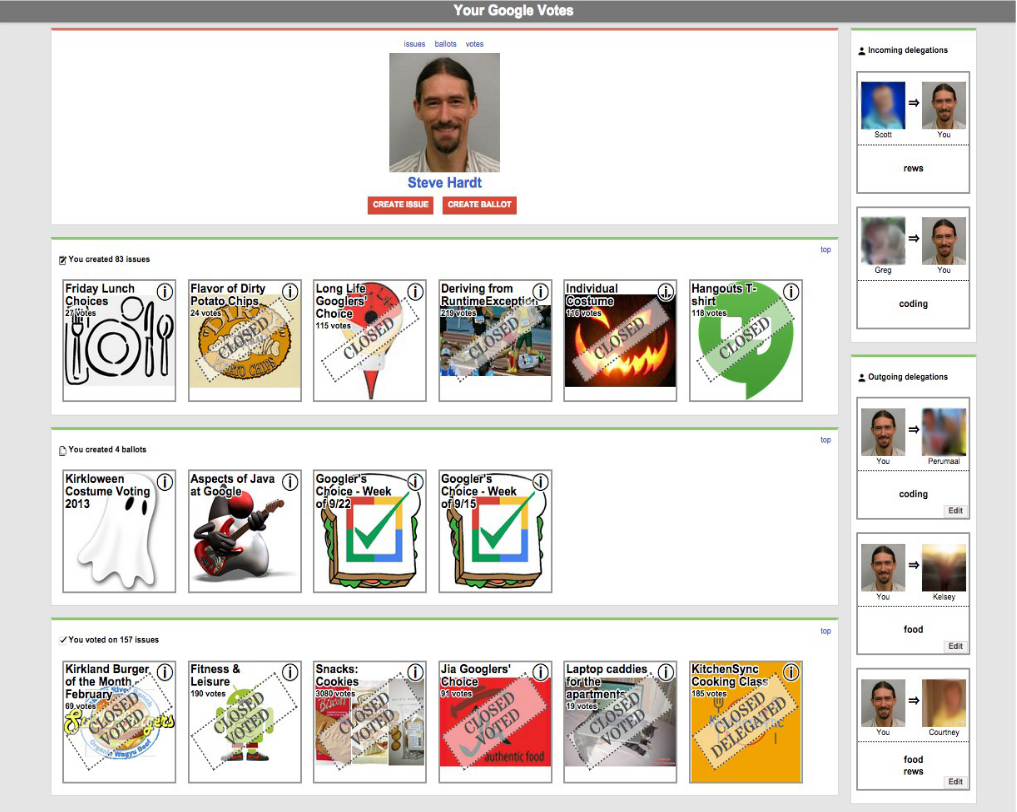
\includegraphics[width=0.8\linewidth]{../common/google_votes.png}
  \caption{Screenshot taken from \citet{hardt_google_2015} showing the user interface of Google Votes.}
\end{figure}

Google Votes was an internal experiment at Google designed to explore the practical application of liquid democracy within a corporate environment. Built on top of the company's internal Google+ social network, it operated between 2012 and 2015 and allowed employees to participate in decision-making by either voting directly or delegating their vote to a colleague \citep{hardt_google_2015}.

Delegations in Google Votes were category-specific, meaning that users could choose different delegates for different areas of interest, such as food, events, or technical infrastructure. These delegations were persistent but could be overridden at any time, giving users flexibility to either rely on trusted experts or vote independently as needed. The system supported transitive delegation and allowed users to reclaim control by casting their own vote, even after delegating.

The platform placed strong emphasis on usability and transparency. Delegation features were rolled out incrementally, with additional tools such as voting power estimates and delegation advertisements helping users understand their influence. One key design principle was what the authors called the ``Golden Rule of Liquid Democracy'': if a user delegates their vote, they should be able to see how it is being used. To accomplish this, users received notifications when their delegate voted, and all votes were visible to the relevant group. This encouraged accountability and gave voters confidence that their delegated votes were being used appropriately.

While Google Votes was never made publicly available, it served as a successful demonstration of liquid democracy in a structured, real-world setting. It showed that being able to delegate votes could improve engagement and decision-making within large organisations, especially when designed with attention to user experience. For vodle, the system provides a concrete example of how features like topic-specific delegation, transparency tools, and real-time voting feedback can make liquid democracy more practical and accessible.
\section{Agent Based Modelling}\label{sec:background_abm}
Agent-based modelling (ABM) is a computational approach used to simulate the actions and interactions of autonomous agents in order to assess their effects on a system as a whole. It is particularly suited for exploring complex, dynamic systems where behaviour emerges from local interactions between individual entities (agents) rather than being dictated by central control. ABM has been widely applied in domains such as economics, sociology, and ecology to study decentralised systems, market dynamics, and collective behaviours \citep{bonabeau2002agent}.

The need to explore ABM arises due to the project's goal of introducing a vote-splitting mechanism that hasn't been explored before into vodle. Traditional analysis alone may not effectively capture the dynamic interactions or unintended consequences that can emerge from this novel feature. Through ABM, it is possible to simulate realistic voting scenarios, track delegation chains, identify potential power imbalances, and anticipate challenges. These simulations can reveal performance insights and inform design decisions before implementing the mechanisms within the live platform.

Several widely used ABM frameworks exist, each with their own strengths and drawbacks relevant to this project:
\begin{itemize}
  \item \textbf{NetLogo} \citep{netlogo} is a highly accessible and widely adopted modelling platform known for its user-friendly graphical interface and ease of learning. It offers rapid prototyping capabilities and excellent visualisation features, allowing clear communication of results. However, very complicated models are not compatible with it.
  \item \textbf{Repast} \citep{repast} provides a powerful and versatile suite of tools for building large-scale, computationally intensive simulations. It supports distributed computing, which is beneficial for extensive delegation networks with potentially thousands of agents. However, Repast has a steep learning curve, which could hinder its compatibility with this heavily time restricted project.
  \item \textbf{Mesa} \citep{kazil_utilizing_2020} is an open-source framework written in Python and specifically designed for agent-based modelling. Its advantage lies in its integration with Python's ecosystem of data science libraries. Simulations built with Mesa can easily make use of tools such as NumPy and pandas for efficient data processing, and Matplotlib or Seaborn for visualising model outputs. This compatibility allows for rapid analysis and iteration, while also significantly lowering the learning curve for developers already familiar with Python. Mesa offers a practical balance between usability and computational flexibility, making it well-suited for customisable and moderately large simulations.
  \item \textbf{Agents.jl} \citep{agentsjl} is a high-performance agent-based modelling framework written in Julia. Due to Julia's speed and efficiency, it is suitable for large-scale and computationally demanding simulations. The framework is designed to be user-friendly, with a syntax that is approachable for those familiar with scientific computing. However, the Julia ecosystem is less mature compared to Python's, which may limit the availability of additional libraries and resources. 
\end{itemize}
Given the time constraints of this project, Mesa offers a practical and efficient solution. Its Python-based interface and straightforward setup allow for rapid development without the overhead of learning a new framework. This ease of use enables more time to be spent designing meaningful experiments and analysing results, rather than configuring tooling.
\section{Vodle}
To effectively explore and implement liquid democracy mechanisms, it is essential to understand the design and technical context of the platform into which they are being integrated. Vodle is a web based decision making tool developed to support participatory group processes through interactive polls and transparent aggregation methods. Its goal is to provide users with flexible, fine grained input mechanisms that encourage compromise between voters, while maintaining accessibility and usability across a broad and diverse user base.

This section introduces the core architecture of vodle, including its underlying rating system (MaxParC) and the technologies that support its operation. These technical foundations were instrumental in shaping the design and feasibility of the advanced delegation features developed in this project. In addition, the platform's design philosophy is examined, providing a basis for the principles that guided the implementation of new components.


\subsection{MaxParC - TODO: rework the summary}
MaxParC (Maximum Partial Consensus) is the core rating system used in vodle to aggregate user preferences and determine poll outcomes. Introduced by \citet{heitzig_fair_2024}, MaxParC was designed to address common limitations of traditional voting systems, particularly the tendency for majority rule to overlook minority preferences. Its goal is to balance fairness, consensus, and efficiency in collective decision-making.

In MaxParC, each user rates an option on a scale from $0$ to $100$. This rating reflects the user's willingness to approve that option based on how many other users also support it. Specifically, a rating of $x$ means that the voter will approve the option if fewer than $x\%$ of participants disapprove. A rating of $0$ means the option is never approved, while $100$ means it is always approved regardless of others' opinions. This structure transforms a simple rating into a conditional approval, allowing for a more nuanced expression of preferences with the potential for compromise.

\begin{figure}[H]
  \centering
  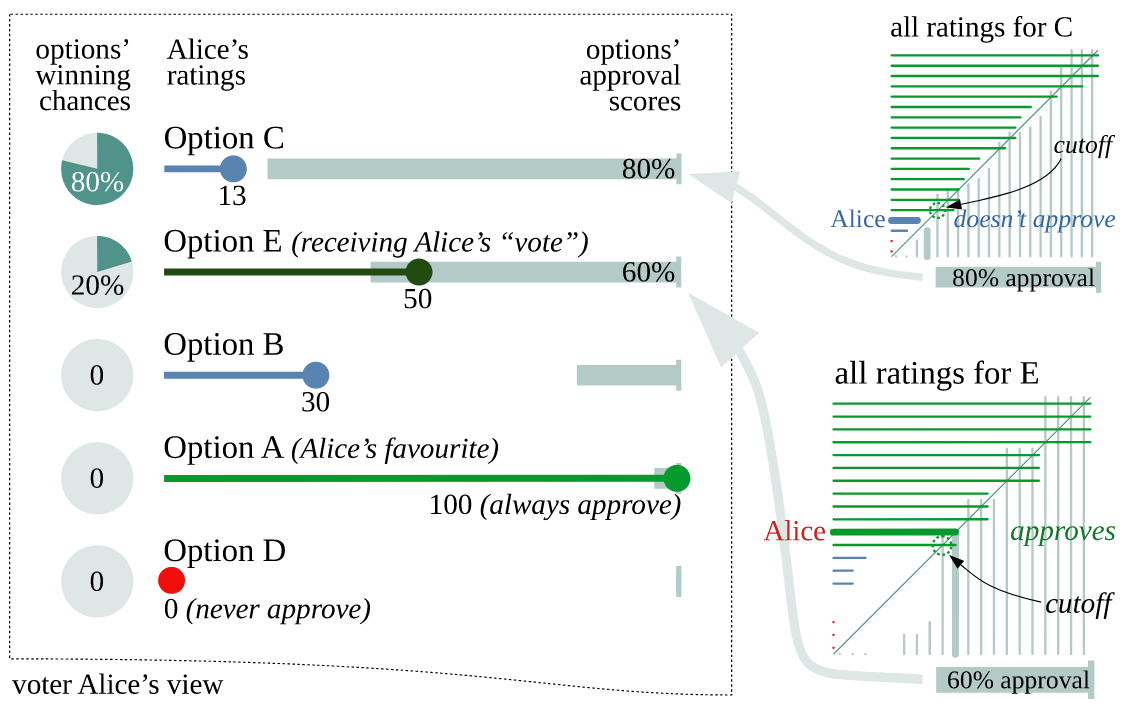
\includegraphics[width=0.8\linewidth]{../common/maxparc.png}
  \caption{Visual representation of MaxParC from the perspective of a voter (Alice). Ratings represent conditional approval thresholds. An option is counted as approved by Alice if the approval bar (light grey) overlaps with her rating needle. Graphic from \citet{heitzig_fair_2024}.}
\end{figure}

\textit{TODO: rework this section to be more concise and clear or remove}
Understanding how MaxParC processes ratings is essential for this project, as the proposed vote splitting mechanism must operate within its conditional approval framework. When a user splits their vote among multiple delegates, the system must ensure that their own rating continues to contribute appropriately. Specifically, if a user delegates $x\%$ of their rating to others, their final rating must not fall below $(100-x)\%$ of their original input. This constraint guarantees that the user's approval remains proportionally represented, even when part of their voting power is passed on to others.

Integrating liquid democracy into vodle therefore requires careful design to align with MaxParC's logic, ensuring both technical compatibility and conceptual consistency.

\subsection{Technologies Used}
Understanding vodle's technology stack is crucial to successfully integrate liquid democracy features into the existing platform. Since the project involves adding complex delegation and voting logic, it's important to appreciate the constraints and benefits of the technologies currently used in vodle, as they directly influence the design and implementation choices.

\subsection*{Angular}
Vodle is built with Angular \citep{angular}, a TypeScript based frontend framework created by Google. Angular's modularity and structured component system provides a strong foundation for incremental development, essential when introducing new features such as ranked delegation that build upon existing components. Its clear separation of concerns helps maintain readable and maintainable code, simplifying debugging and future enhancements. This is particularly beneficial as the delegation logic is expected to grow in complexity and build upon existing components as the project progresses.

\subsection*{Ionic Framework}
The Ionic \citep{ionic} framework complements Angular by enabling the creation of responsive, mobile-compatible applications from a single codebase. Given vodle's goal of broad user participation, Ionic ensures that its functionalities remain consistent and accessible across both desktop and mobile devices. %need to make sure its compatible 
For this project, new delegation features must be designed to work seamlessly within the existing Ionic framework, ensuring that they are visually appealing and user-friendly on all platforms, including mobile devices.

\subsection*{CouchDB}
CouchDB \citep{couchdb} is vodle's primary data storage method and communicates directly with the client through HTTP requests, meaning there is no dedicated backend. This architecture places significant computational responsibilities on the client-side Angular application, including the handling of delegation chains, cycle detection, and the computation of final vote outcomes. Furthermore, since CouchDB stores data exclusively as JSON-formatted strings, complex delegation structures and voting relationships must be serialised and de-serialised on the client side.

The lack of server-side computation means the delegation algorithms must be designed with client-side efficiency in mind, ensuring performance remains acceptable even as delegation complexity increases. Thus, the choice of algorithms for liquid democracy features, such as those to resolve conflicting delegation paths, is directly influenced by CouchDB's architectural constraints.

These technological considerations (covered in more detail in Section~\ref{sec:design_architecture}) strongly shaped the practical implementation of liquid democracy in vodle. They necessitated a focus on efficient client-side logic as well as careful management of data flow.

\subsection{Partially Implemented Delegation in Vodle}\label{subsec:background_existing_delegation}
Vodle contained an incomplete implementation of vote delegation at the beginning of the project. While this functionality was not exposed to end users and had never been deployed in a working state, several components of a delegation system were already present in the codebase. These included an invitation based mechanism for creating delegations, along with the user interface elements required for it to function.

This implementation also attempted to prevent delegation cycles, but its behaviour was inconsistent. Because delegation graphs were stored only in local memory and not synchronised across clients, different browsers could have divergent views of the delegation state. As a result, delegation actions that passed cycle checks on one client could fail on another, undermining the reliability of the system.

Although inactive and incomplete, this partial implementation helped clarify some of the challenges involved in integrating liquid democracy into vodle -- in particular those related to consistency, synchronisation, and user experience. It also provided a foundation of interface patterns and conceptual models that were built upon the development of the project.

Further discussion of the issues with this implementation as well as how it was adapted, improved, or replaced can be found in Chapter~\ref{ch:design_implementation}.
\subsection{Design Philosophy}


\section{Summary}
The background research presented in this chapter has provided the necessary foundation for designing and implementing advanced delegation features within vodle. Initially, the research highlighted critical limitations in traditional liquid democracy systems, such as the formation of delegation cycles, the risks associated with abstentions, and the disproportionate influence of super-voters. These insights showed the need for implementing delegation mechanisms that are capable of addressing these challenges effectively.

Research into these mechanisms revealed several promising methods. Ranked delegation was found to be an effective approach for reducing the risk of lost votes, with the MinSum delegation rule being particularly suitable due to its clear balance of efficiency, interpretability, and fairness. Vote splitting was identified as a valuable strategy to allow voters greater flexibility by distributing their influence among multiple trusted delegates. Additionally, the concept of delegating different options to distinct delegates was supported by practical experiences from Google Votes, where topic-specific delegations improved user engagement and representation accuracy.

Among the vote splitting methods explored, the trust matrix model stood out for its expressiveness and alignment with vodle's goals of user autonomy and flexibility. By allowing voters to articulate nuanced trust relationships across multiple delegates, including themselves, the model offers a compelling balance between representation quality and individual control. While more computationally intensive than simpler approaches, it presents a viable strategy for robust vote splitting within a real-time voting system.

The technological constraints of vodle itself, especially the reliance on client-side processing due to the CouchDB architecture, demonstrated the need for efficient, lightweight implementation strategies.

These insights collectively define the project's objectives, which are formalised in the following chapter. The objectives are designed explicitly to address the limitations uncovered in the research, ensuring the integration of liquid democracy into vodle is practical, user-friendly, and aligned with established best practices.